\section{Toward an Sequence of Target Poses}
\label{section: toward_sequence_target_poses}
In previous section motion and manipulation planning, planning for a single action was discussed, feasibility of a path depends on local planners in the form of predictors provided by system models discussed in \cref{chapter: interaction_with_env_and_model_identification}. In this section planning for a longer horizon is discussed, \textit{task planning}. As a reminder, a task was defined as a set of objects with associated target configurations. Task planning is defined as the following arisen problem. When given a task, which actions should successfully be performed and in which order to fulfil the given task. Finding such an action sequence in an environment with movable obstacles bears the name \ac{NAMO}. An example is given in \cref{figure: example_task_planning} and serves to clarify the planning problem. In this example the robot is tasked with placing the cube on the location where the sphere currently is.\\

A possible action sequence manually derived would be:\\

\begin{enumerate}
\item drive toward the ball
    \item if no system model is available, perform system identification on the ball
    \item push the ball away such that the box's target position is free 
    \item drive toward the cube
    \item perform system identification on the cube 
    \item push the cube to the target location
    \end{enumerate}
    
\begin{figure}[H]
    \centering
    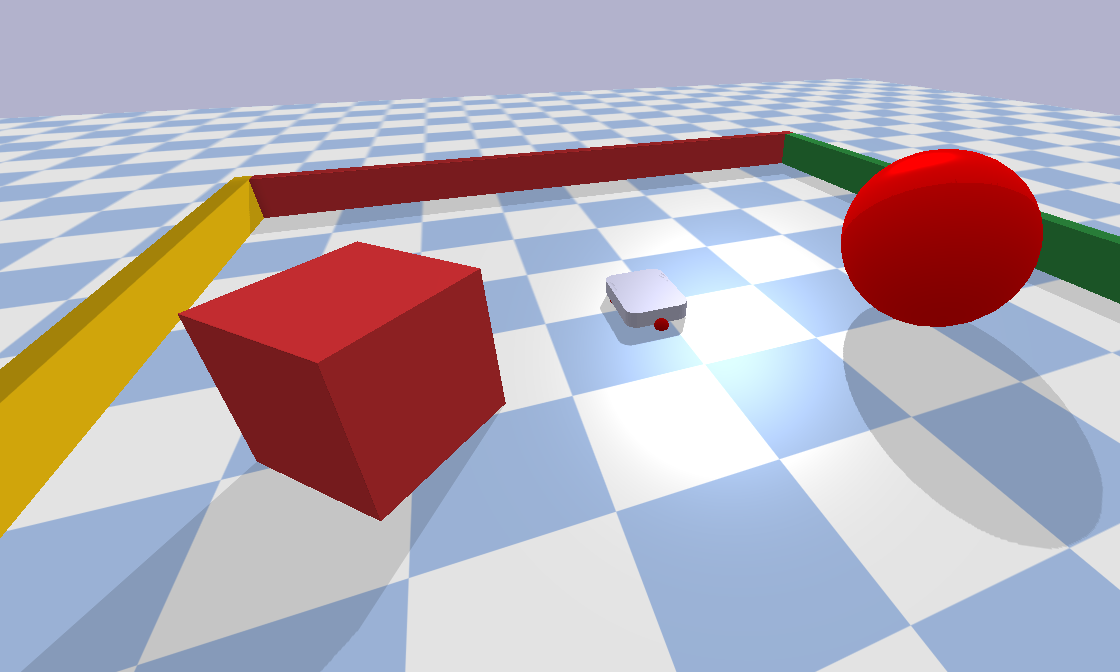
\includegraphics[width=0.6\textwidth]{figures/task_swap_location_balls.png}
    \caption{Example environment with robot, a sphere- and cube object and unmovable walls. The robot is tasked with pushing the cube to the location where the sphere currently is }
  \label{figure: example_task_planning}
\end{figure}

Essentially the task planners job is to create an action sequence, containing subtasks in a logical order which fulfils a larger given task. The task planners reviewed in this literature study fall in to one of the 3 categories: a high-level planners, planning in a joint configuration space and hierarchical planners. Task planners can validate a single motion by querying a motion planning algorithm, discussed in \cref{subsection: motion_planning}. Motion planning algorithms can be queried resulting in a path or the message a path cannot be found, from the perspective of the task planner it appears thus that motion planning is decidable even though it may sometimes given an incorrect answer. 

\subsection{Arisen Problems with Task Planning with Movable Obstacles}
\label{subsection: problems_with_task_planning}
Before diving into arisen problems, the joint configuration space and the piecewise-analytic configuration space are defined. A \textit{joint configuration space} of the robot and the obstacles is created by augmenting the robot configuration space with every configuration space for all objects. For example, if the configuration space for both robot and objects consist of position $X$, $Y$ and orientation $\theta$, then the joint configuration space is $3n$-dimensional, where $n$ is the number of objects including the robot. When the robot manipulates an object, certain multi-body constraints are applicable and are different from single-body constraints, a configuration space containing multiple modes where different constraints apply is called an \textit{piecewise-analytic} configuration space \cite{goldberg_asymptotically_2020}. The joint configuration space with multiple modes of dynamics is an example of a piecewise-analytic configuration space.\\

In this literature, the task planner must solve a \ac{NAMO} problem with unknown but learnable true dynamics. Directly planning in joint configuration space of the robot and objects is tedious for \ac{NAMO} because of different modes of dynamics. For example, the robot can be driving, then pushing and then driving. The push action influences the free space where the robot has to drive in if the push manipulation has ceased. With multiple objects, directly planning in a joint configuration space causes a exponential number of possibilities. \\

With a given task, the target poses of certain objects are given, but that does not specify the location of other objects which may be present in the environment, such as the location of the sphere in the example displayed in \cref{figure: example_task_planning}. If the final positions of some objects are unspecified, this leads to problem dimensionality that is exponential in the number of objects with unspecified target positions in the environment \cite{scholz_navigation_2016}, and is known to be NP-hard \cite{reif_motion_1985}.\\

The two reasons above are indicating the challenges an task planner is facing when solving the \ac{NAMO} problems, both planning in a piecewise-analytic configuration space and trying to solve an NP-hard problem also occur with known dynamics. This literature assumes unknown objects, single-body systems dynamics are a priori not or party known, a priori the dynamics of multi-body systems are unknown. Thus planning has to be performed with learned dynamics which is important to keep in mind, because of estimations of the true dynamics motion and manipulation planning might return unfeasible paths, and feasible paths might not be found. Compared to known dynamics, learned dynamics adds a large layer of uncertainty to the \ac{NAMO} problem.\\

\subsection{Planning in Joint Configuration Space}
\label{subsection: planning_in_joint_config}
As already indicated in \cref{subsection: problems_with_task_planning}, the joint configuration space's dimensionality grows linearly, meaning the joint configuration space grows exponentially in the number of objects, which is an explosion in the number of possible combinations the environment can be in. Even sampling cannot computationally find a path in reasonable time, only by leveraging simplifications a search be performed. The upcoming solutions to search in the joint configuration space all implement some simplification to prevent sampling the entire joint configuration space. \\

Note that while other task planning methods might use motion/manipulation planning to validate motions/manipulations, planning in joint configuration space does not. Planning in joint configuration space essentially is motion/manipulation planning for a longer horizon than a single action.\\

Novin \cite{sabbagh_novin_optimal_2016} develops a task planner for the \ac{NAMO} problem combined with placing objects on target positions which is capable of finding a local minimum in the joint configuration space. Tackling the combinational explosion using 2 different tactics, first, a disjunctive programming concept is applied to convert the continuous problem to discrete form, where a continuous path is equivalent to some points with equal time distance in between, second, a heuristic function is implemented, which allows for planning toward the goal for a fixed number of time steps. Such a receding horizon allows only to search a path close to the current joint configurations. Planning toward configurations lowering a metric function indicating the direction toward the final target configuration. Convex optimisation then finds an optimal path regarding the considered horizon \cite{sabbagh_novin_optimal_2016}. Novin then finds the \ac{NAMO} problem while learning dynamical properties in a hospital setting. Where patients are assisted by the patients' assistant mobile robot which can move obstacles out of the way or hand patients their walker. In addition to the task planner, a Bayesian regression algorithm was used to estimate the object dynamical model and an \ac{MPC}-based controller was used to follow a specified path \cite{novin_dynamic_2018}. In a follow-up paper, trajectory errors have been lowered and the selection of objects to encounter has been enlarged \cite{sabbagh_novin_model_2021}. Novin has shown that by sampling close to the current configuration, a path can be found in high dimensional configuration spaces in reasonable time. The patient assistant mobile robot is able to find and track a path in real-time.\\

\cite{goldberg_asymptotically_2020} solves the \ac{NAMO} problem by first extending existing algorithms developed by \cite{hauser_randomized_2011} to an optimal but prohibitively computationally expensive algorithm. Then the configuration space is factored while preserving optimality, this reduces the complexity considerably, by considering only a finite collection of subsets of the configuration space, each of which is subject only to analytic constraints. By building a graph on each of these subsets and connecting the resulting collection of graphs, we can construct a random graph that spans the configuration space. As the collection grows sufficiently large, it will contain a near-optimal plan with probability one and an optimal plan in the limit of infinite samples. \\

The 2 papers discussed have shown that the computational nightmare of the joint configuration space can be tamed by techniques such as discretization, factorization or a heuristic function combined with a time horizon. Such techniques prevent searching in configurations relatively far from the current configuration, while optimality guarantees can be given and real-time implementations have been shown. A relief bonus for solving the \ac{NAMO} problem in the joint configuration space which requires much computation power is that it removes the need for individual motion or manipulation planning. It can be concluded that if clever techniques keep the dimensionality to an reasonable small subspace, such that the robot can start tracking a path in under a minute of searching, path searching in the joint configurations space is a successful methods for task planning.\\

\subsection{High-level Planners}
\label{subsection: high_level_planners}
\textit{High-level planners}, in this literature refers to an ontology defining the structure of knowledge in a certain domain and a planner which when queried with a task or question uses the ontology to derive an answer or action sequence. Advanced high-level planners automatically try to satisfy 'logical' constraints that for humans feel obvious such as holding a cup upright if it is filled with liquid. A summary of high-level languages, planners and frameworks specialised for robotic applications will now be discussed, for this discussion, the literature study of M. Mâachou has been used containing a recent summary of the high-level planners \cite{maachou_mohommed_knowledge-based_2021}. \\

Note not all high-level planners \textit{must} use an \textit{ontology}, many however do, to categorise objects and actions as concepts, roles and instances. An example concept is the set of mobile robots with grippers, Tiago (a mobile robot with grippers) is an instance of the concept mobile robots with grippers, $\text{apple}_1$ is an instance of the concept fruit and can be gripped by Tiago, then the role Tiago.canGrab($\text{apple}_1$) indicates that Tiago can grab $\text{apple}_1$. Ontologies create hierarchical categorisations for example, a categorisation of products in a supermarket where chocolate croissant is a subconcept croissant, a subconcept of bread. Most popular languages to store an ontologies are the \ac{PDDL} and the \ac{OWL}. Ontologies cannot categorise and relate every action, concept or physical object existing in the real world, that is way too much data. That is why ontologies are specific to a certain domain such as a supermarket environment, an hospital environment or a family home. Large domain-specific ontologies are available open-source, for robotics applications the most popular ontologies are \ac{SUMO}, \ac{CORA} and \ac{DOLCE}. \\

Ontologies are deterministic, the closed-world assumption (note, not the same assumption as assumption \ref{assumption: closed_world}) is used to make unknown statements decidable, the closed-world assumption states, anything not known to be true is assumed to be false. While learning dynamical properties many statements are unknown, with the closed-world assumption high-level planners mainly would assume manipulation to be impossible, for example, if the high-level planner is queried with "can the unknown object be moved", the answer would simply lead to false because it is unknown. Here \textit{affordances} can help to make an estimation, affordance is defined as the ability to perform a certain action with an object in a given environment \cite{ardon_affordances_2020}. Concluding that a certain manipulation action would lead to success with an unknown object requires some experience before any conclusion can be drawn. Actions which collect experience for a given object should be triggered in high-level planners to update the knowledge base which then bypasses the closed-world assumption. \\

Frameworks (which include a ontology, planner and more) such as KnowRob \cite{beetz_know_2018} or the perception and manipulation knowledge  \cite{diab_pmkknowledge_2019} show the effectiveness of high-level planners in robotic applications. \\

High-level planners in practice are successful in generating an action sequences, however, in the scope of this literature study, where tasks are defined as a set of objects with target configurations high-level planners are not needed. There is not classification of objects required, no distinction between physical places such as kitchen and living room. An high-level planner in the scope of this literature is thus overkill. Simple heuristic and flowchart like decisions trees, see \cref{figure: navigation_algorithm} achieve the same performance as expensive planners, thus the former is preferred. 

\begin{figure} \centering
\begin{tikzpicture}[node distance = 2cm, auto]
    % Place nodes
    \node [block] (global) {Global Path};
    \node [decision, below of=global] (obstacle) {Obstacle Detected};
    \node [block, below of=obstacle, node distance=3cm] (generate) {Generate Obstacle};
    \node [decision, below of=generate] (movable) {Movable};
    \node [block,  left of=movable, node distance=3cm] (remove) {Remove Obstacle};
    \node [block,  right of=movable, node distance=3cm] (replan) {Replan Path};
    % Draw edges
    \path [line] (global) -- (obstacle);
    \path [line] (obstacle) --  node [near start] {yes} (generate);
    \path [line] (obstacle.west) -| ($(obstacle.west) - (1,0mm)$) |-  node [near start] {no} (global.west);
    \path [line] (generate) -- (movable);
    \path [line] (movable) --  node [near start, above] {yes} (remove);
    \path [line] (movable) --  node [near start] {no} (replan);
    \path [line] (remove) |- (global);
    \path [line] (replan) |- (global);
\end{tikzpicture}
\caption{Flowchart representation of navigation algorithm \cite{wang_affordance-based_2020}}
\label{figure: navigation_algorithm}
\end{figure}


\subsection{Hierarchical Planning}
\label{subsection: hierarchical_planning}
Hierarchical planners separate the robot's configurations space into subspaces. In such graphs where the subspace is a section where a single dynamical mode holds true, such as driving, pulling or pushing. During seperations into subspaces, actions are generated and a graph (such as a \ac{MDP} or search tree \cite{bronson_practical_2010}) combines actions with subspaces, where the nodes correspond to robot and object poses, and transitions to actions. Solving a task planning problem is then defined as finding a list of transitions which start in the current configuration (contained inside a subspace) and end in the target configuration (inside a subspace), an example is displayed in \cref{figure: example_hierarchical_planning}.\\

\begin{figure}[!h]
    \centering
    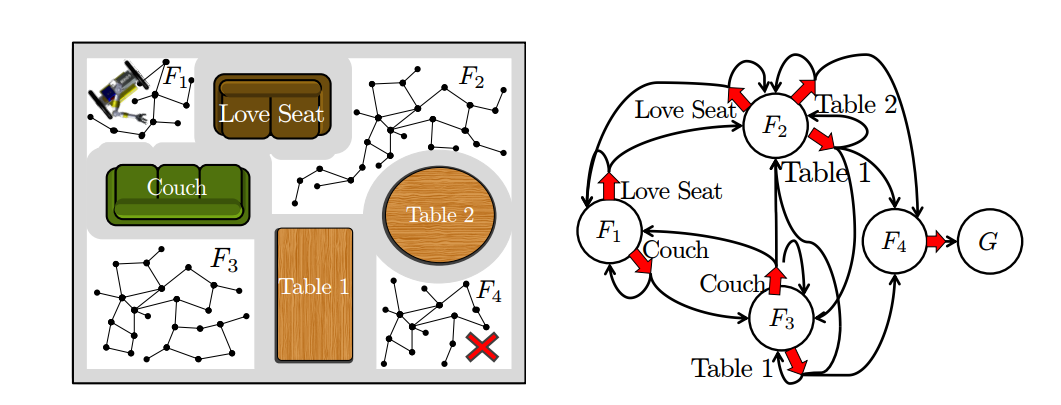
\includegraphics[width=0.9\textwidth]{figures/construct_hierarchical_planner.png}
    \caption{Schematic overview of the robots' free space separated is subgraps in \acs{PRM} and the corresponding \acs{MDP}, from \cite{scholz_navigation_2016}
    }
    \label{figure: example_hierarchical_planning}
\end{figure}

\Cref{figure: example_hierarchical_planning} displays a schematic overview of a separated configuration space of the robot, free space is made into 4 subspaces, $F_1$, $F_2$, $F_3$ and $F_4$. Detecting subspaces is found by finding disconnected connectivity graphs after a limited number of samples, and objects inbetween disconnected graphs can be extracted based on position relative to the sampled configurations. An \ac{MDP} can then be constructed and is viewed as a reward shaping mechanism to focus the low-level search on actions that are likely to clear paths to useful locations \cite{scholz_navigation_2016}. Solving the \ac{MDP} generates multiple ordered action sequences which would lead to the robot's target configuration. \\

Task planning with learned dynamics was first done by Scholz \cite{scholz_navigation_2016}, the work has inspired \cref{figure: example_hierarchical_planning} and it was the first attempt to solve the \ac{NAMO} using learned dynamics \cite{scholz_learning_2015}.  By using a hierarchical \ac{MDP} formulation of the \ac{NAMO} problem designed to handle dynamics uncertainty, Scholz successfully demonstrated the ability of a robot to adapt to unexpected object behaviour such as a table which upon inspection turned out to be unmovable. A key difference between Scholz task description and this literture review's task description is that in \cite{scholz_navigation_2016} the target position for only the robot is given, where as this literature includes possibly some target positions for objects. Including target positions for the obstacles makes such a problem quite a bit harder since additional planning is required, it is then unclear if such a problem can be solved using sampling algorithms combined with an \acp{MDP}.\\

Instead of defining actions and subgraphs as previously shown, \textit{backward induction} determines the actions, and applies them to the target configuration to search for the starting configuration. An arisen problem is the unspecified target positions of the objects in the environment. A workaround is to simplify the \ac{NAMO} problem to object rearrangement for which all start and target configurations are specified. Krontiris and Bekris created such conditions in object rearrangement problem in which object move over a straight line, and can only be moved once (monotone problem) \cite{krontiris_dealing_2015}. A graph is created where nodes corresponding to the objects pose in the world. From target node to the current node is searched in a backwards fashion. With the monotone rearrangement search algorithm constructed by \cite{krontiris_dealing_2015} finding a solution is sublinear in the number of objects to rearrange and the algorithm is run-time applicable. \\

Generally target positions other than the robot itself are not specified in \ac{NAMO} problems. Unspecified target positions can be randomly chosen, as \cite{siciliano_path_2009} has shown. By augmenting a search tree with manipulated objects to random locations, a special feature is that \cite{siciliano_path_2009} keeps track of the robot and object configurations within the search tree. Randomly selected actions applied to randomly chosen actions guarantees probabilistic completeness for infinite sampling, but the computational power required increases drastically with the size of the number of objects and size of the workspace (and thus directly configurations space). Heuristic functions could potentially prevent unnessecary sampling into unrelevant subspaces of the configuration space, such as \cite{sabbagh_novin_model_2021} has shown.\\

Heuristic task planners find solutions which are \textit{hierarchical}, they will return the best feasible plan that can be expressed within the task hierarchy they search \cite{goldberg_asymptotically_2020}. System models contain some model mismatch with the true dynamics. Both the hierarchical solutions and effects of model mismatch are acceptable mainly because the \ac{NAMO} problem is NP-hard. Hierarchical planners are relatively computationally efficient, compared to planning in joint configuration space and find a action sequence (even though that might be hierarchical). It can be concluded that hierarchical planners are thus a right fit to determine action sequences in the scope of this literature. \\

\section{Discussion}
\label{section: tamp_discussion}
sample- and graph based motion and manipulation planning algorithms have been discussed, the most applicable motion planning algorithms are the sample-based algorithms because they can search high dimensional spaces efficiently compared to graph-based planners. a connectivity graph build on sampled configurations indicates if samples are reachable from other sampled configurations while satisfying constraints imposed by the local planner. Feasibility has been shown to depend on local planners, who's accuracy directly depends on system models discussed in previous chapter. both path existence and convergence properties have been discussed, which allows to conclude that sample-based planners can efficiently search for motion and manipulation problems, additional checks such as path existence can speed up arriving to conclusions, such as "no path exists". \\

The joint configuration space is a piecewise-analytic configuration space containing multiple modes of dynamics. Because this joint configuration space dimensionality grows linearly (and the configurations space thus exponentially) with the number of objects, it is computationally infeasible to search for a path. Especially considering that with robotic application  solutions found in real-time are highly appreciated. The exponentially fast growing joint configuration space is an answer to the second research subquestion. \\

Three main methods have been discussed to determine an action sequence to reach a given task, firstly planning in a joint configuration space where the dimensionality grows so enormously fast that measures have to be taken in order to make the problem computable. Using techniques such as discretisation, a finite planning horizon or factorisation decrease the search space such that real-time planning is possible, allowing to conclude that planning in joint configuration space is effective, and applicable for task planning with learned dynamics. Secondly, high-level planners, which with an ontology and planner determine an action sequence. The task is defined as a set of object and corresponding target configurations, this form of task and the lack of categorisation of objects yields high-level planners shy of providing effective solution. To conclude high-level planners are not fit for determining a action sequence in this literature. The last methods is hierarchical planning, by seperating the joint configuration space in local subspace where one mode of dynamics holds, motion planning algorithms can find a paths in these subspaces, a global plan is found by generating a search tree or \ac{MDP} from planning to target. The solutions found are hierarchical, which limits converging to a global minimum, even so the methods is efficient compared to a search into joint configuration space. With learned, possibly inaccurate dynamical models, converging toward the optimal path is not the goal of the task planner, and hierarchical solutions with computational efficiency are preferred, allowing to conclude that hierarchical solutions are effective and applicable approach to find an action sequence for tasks to execute in an environment with movable obstacles.\\ 